\documentclass[12pt,letterpaper]{article}
\usepackage[utf8]{inputenc}
\usepackage[spanish]{babel}
\usepackage{graphicx}
\usepackage[left=2cm,right=2cm,top=2cm,bottom=2cm]{geometry}
\usepackage{graphicx} % figuras
% \usepackage{subfigure} % subfiguras
\usepackage{float} % para usar [H]
\usepackage{amsmath}
%\usepackage{txfonts}
\usepackage{stackrel} 
\usepackage{multirow}
\usepackage{enumerate} % enumerados
\renewcommand{\labelitemi}{$-$}
\renewcommand{\labelitemii}{$\cdot$}
% \author{}
% \title{Caratula}
\begin{document}

% Fancy Header and Footer
% \usepackage{fancyhdr}
% \pagestyle{fancy}
% \cfoot{}
% \rfoot{\thepage}
%

% \usepackage[hidelinks]{hyperref} % CREA HYPERVINCULOS EN INDICE

% \author{}
\title{Caratula}

\begin{titlepage}
\begin{center}
\large{UNIVERSIDAD PRIVADA-DE-TACNA}\\
\vspace*{-0.025in}
\begin{figure}[htb]
\begin{center}

\includegraphics[width=8cm]{./Imagenes/logo}
\end{center}
\end{figure}
\vspace*{0.15in}
INGENIERIA DE SISTEMAS  \\

\vspace*{0.5in}
\begin{large}
TITULO:\\
\end{large}

\vspace*{0.1in}
\begin{Large}
\textbf{INFORME DE LABORATORIO No 04 -  Crear una Dimensión Regular con SQL Server Analysis Services
Analysis Services}\\
\end{Large}

\vspace*{0.3in}
\begin{Large}
\textbf{CURSO:} \\
\end{Large}

\vspace*{0.1in}
\begin{large}
INTELIGENCIA DE NEGOCIOS\\
\end{large}

\vspace*{0.3in}
\begin{Large}
\textbf{DOCENTE(ING):} \\
\end{Large}

\vspace*{0.1in}
\begin{large}
 Patrick Cuadros Quiroga\\
\end{large}

\vspace*{0.2in}
\vspace*{0.1in}
\begin{large}
Estudiante: \\ 
Sharon Sosa Bedoya          (2016054460) \\
\end{large}
\end{center}

\end{titlepage}


\tableofcontents % INDICE
\thispagestyle{empty} % INDICE SIN NUMERO
\newpage
\setcounter{page}{1} % REINICIAR CONTADOR DE PAGINAS DESPUES DEL INDICE

\section{INFORMACIÓN GENERAL} 

\begin{itemize}
\subsection{Objetivos:}
	\item Crear una Dimensión sobre un Cubo Multidimensional en SQL Server Analysis Services para que usuarios finales puedan explotar la información

\subsection{Equipos, materiales, programas y recursos utilizados:}
	\item Windows 10 64bit: Pro, Enterprise o Education, con al menos 4GB de RAM.
	\item Base de datos AdventureWorksLT2012 r
	\item Tener los archivos de recursos del laboratorio.
	\item Microsoft SQL Server 2017 o superior
	\item SQL SERVER Integration Services

\end{itemize}

\section{PROCEDIMIENTO} 

\begin{itemize}
\subsection{Creación de una Dimensión Regular}
	 \item  En el Solution Explorer nos ubicamos en Data Sources View y podemos ver que tenemos la vista de las
siguientes tablas:
	\begin{center}
	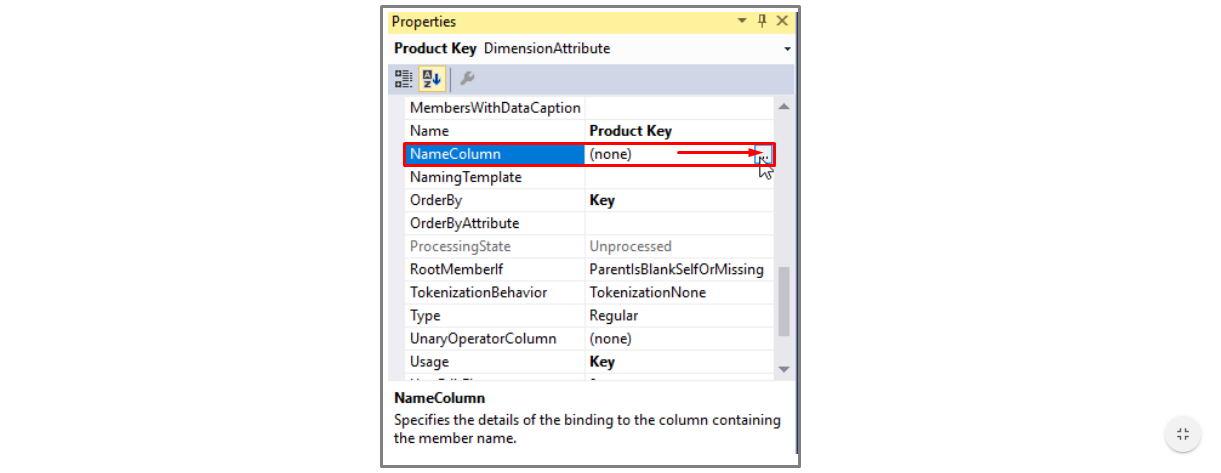
\includegraphics[width=\columnwidth]{./Imagenes/img1}
	\end{center}	


 \item Siempre se recomienda primero crear las dimensiones y como paso final recién crear el cubo, es por eso que
eliminamos el cubo creado en el primer post. Luego nos dirigimos a Dimensions. Click derecho y ubicamos
New Dimension
	\begin{center}
	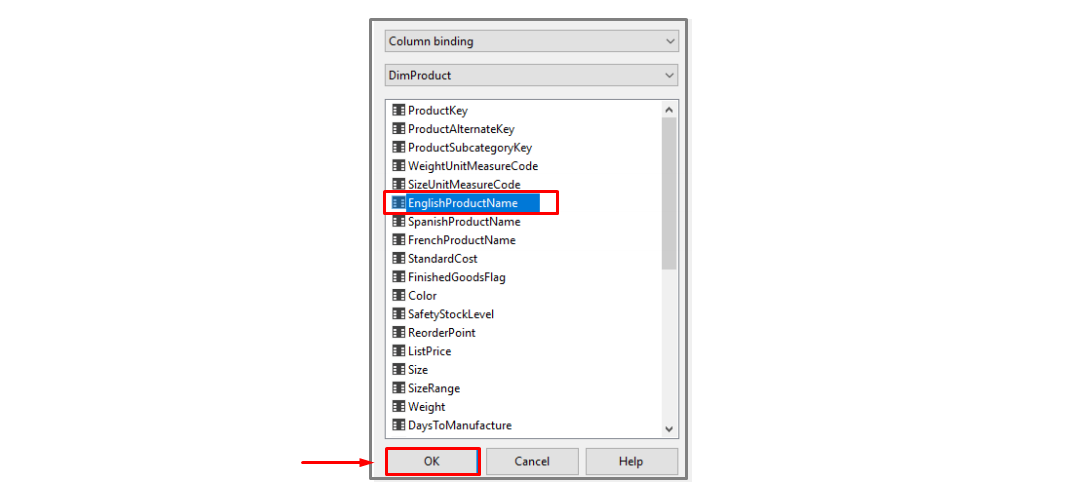
\includegraphics[width=\columnwidth]{./Imagenes/img2}
	\end{center}	

 \item Nos abrirá un Wizard, donde la primera ventana es un resumen de lo que se puede realizar.
	\begin{center}
	
\includegraphics[width=\columnwidth]{./Imagenes/img3}
	\end{center}	

 \item Esta paso en el wizard es muy importante ya que nos permite seleccionar el origen de la dimensión a crear.
Seleccionamos la primera opcion:
	\begin{center}
	
\includegraphics[width=\columnwidth]{./Imagenes/img4}
    \end{center}	

 \item Seleccionamos el Data source view (podríamos tener más de uno) y la tabla Dimensión, en este ejemplo
DimProduct. En Key columns por defecto siempre selecciona al Primary Key de la tabla, pero este valor luego
podría ser cambiado. También podemos añadirle un Name Column a este Key column pero lo dejaremos tal
como esta:
    
	\begin{center}
	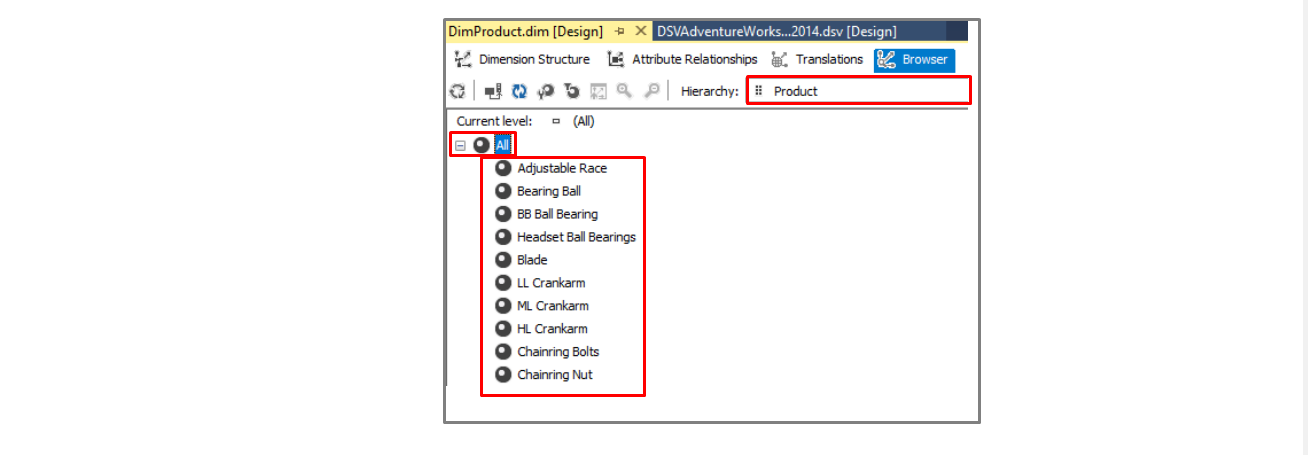
\includegraphics[width=\columnwidth]{./Imagenes/img5}
    \end{center}	
 \item Marcamos los atributos con los cuales trabajaremos:
    
	\begin{center}
	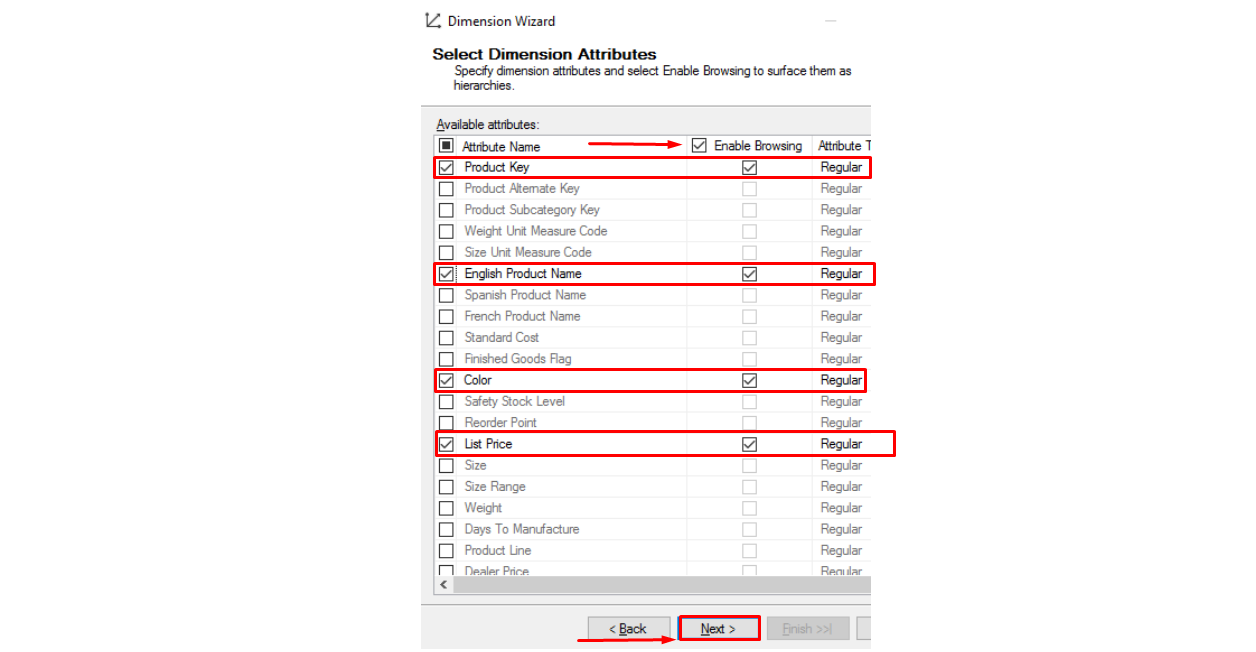
\includegraphics[width=\columnwidth]{./Imagenes/img6}
    \end{center}	
 \item Indicamos el Nombre a la dimensión:
	\begin{center}
	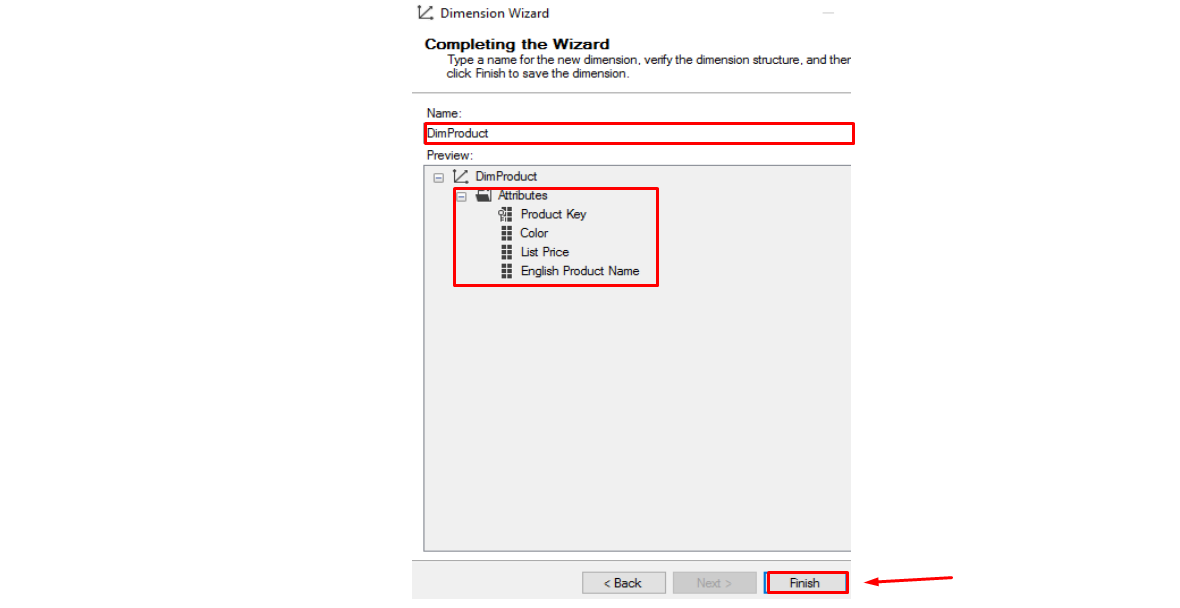
\includegraphics[width=\columnwidth]{./Imagenes/img7}
    \end{center}	

\subsection{Procesar una Dimensión}

	 \item  Ya creada la dimensión, el siguiente paso es Procesarla para ver la generación de los datos. En la pestaña
de Dimension Structure ubicamos la opción de Process:

	\begin{center}
	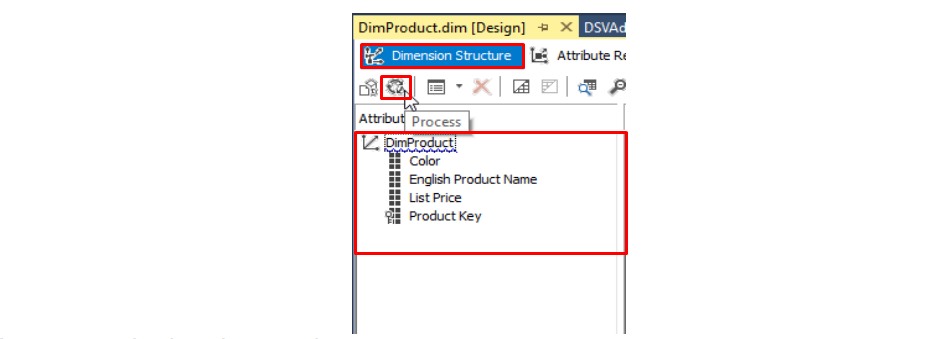
\includegraphics[width=\columnwidth]{./Imagenes/img13}
	\end{center}
\item  Se nos abrirá una ventana donde nos mostrará el progreso del proceso de la dimensión DimProduct:
	\begin{center}
	
\includegraphics[width=\columnwidth]{./Imagenes/img17}
    \end{center}	
    

\item  En la pestaña de Browser exploramos los atributos y los valores que contienen.
Exploramos el atributo Color:

	\begin{center}
	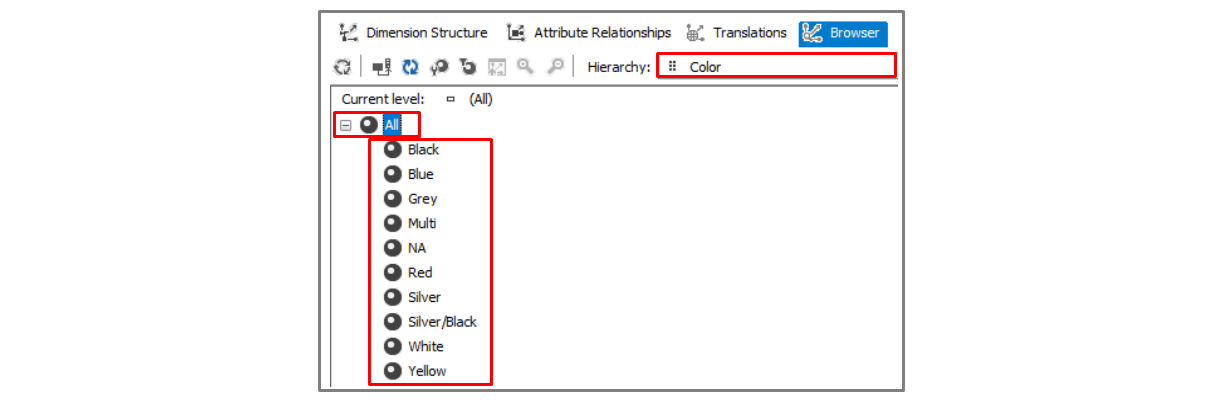
\includegraphics[width=\columnwidth]{./Imagenes/img19}
    \end{center}	
    
\item  Exploramos el atributo English Product Name:
    \begin{center}
	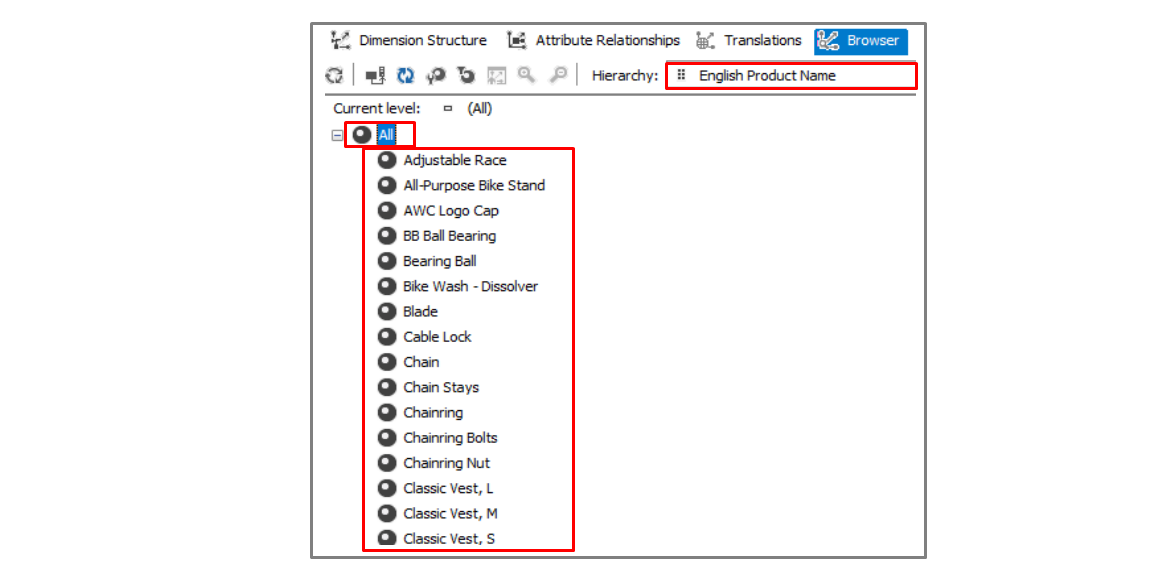
\includegraphics[width=\columnwidth]{./Imagenes/img21}
    \end{center}	
 
\item  Exploramos el atributo Product Key:

	\begin{center}
	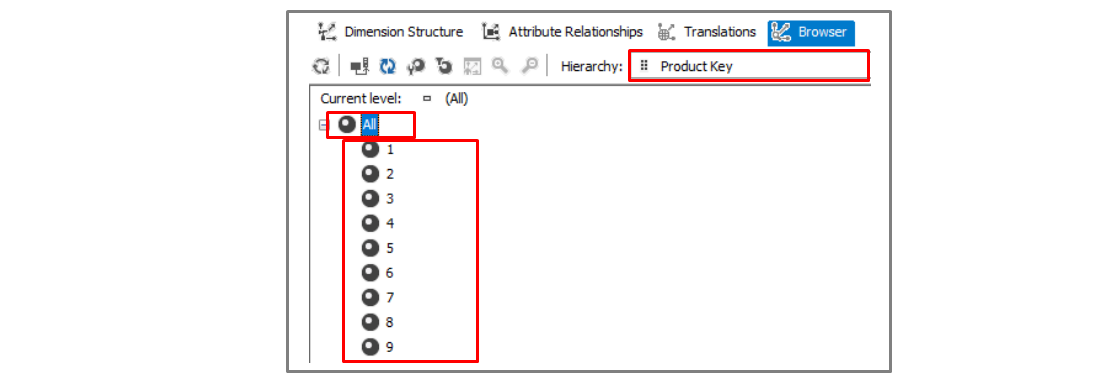
\includegraphics[width=\columnwidth]{./Imagenes/img22}
    \end{center}	
   
Es aquí donde detectamos que si bien es cierto nos muestra los valores de Product Key , lo recomendable
es que este atributo no sea visible para el usuario final, ya que esta es una llave propia del DW.

\subsection{Creación de un Cubo}


\item En las propiedades del atributo Product Key nos ubicamos en NameColumn:

	\begin{center}
	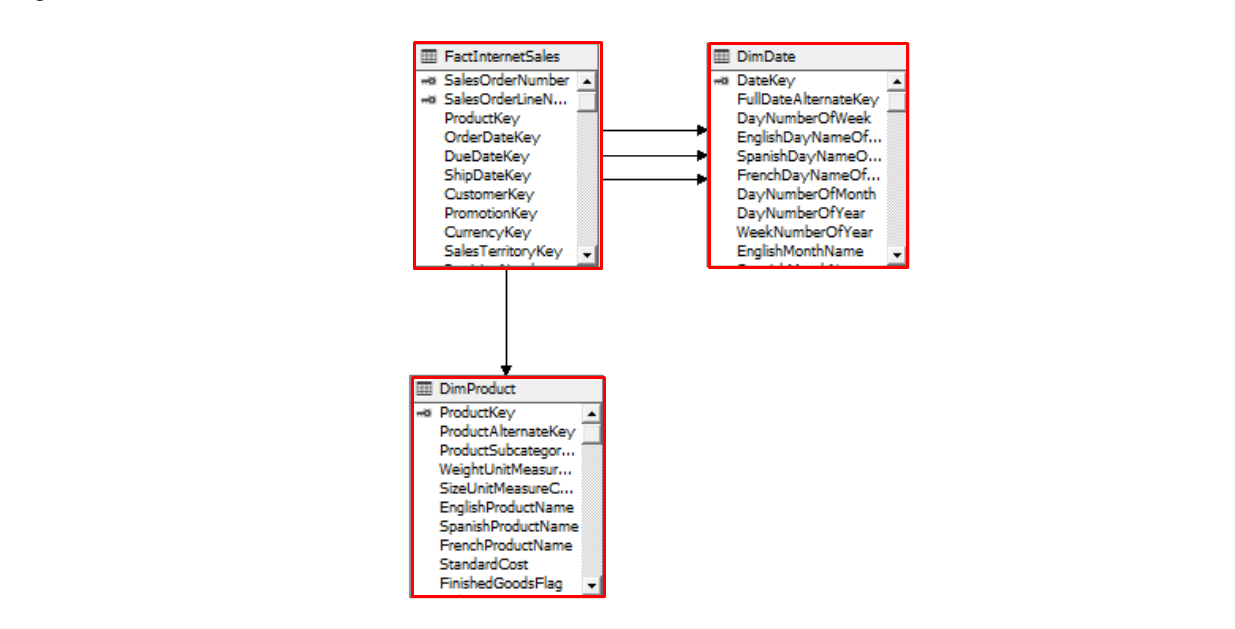
\includegraphics[width=\columnwidth]{./Imagenes/img1_3}
	\end{center}	

\item Nos abrirá una ventana donde podemos enmascarar este atributo por otro, en este caso seleccionaremos el
atributo EnglishProductName:

	\begin{center}
	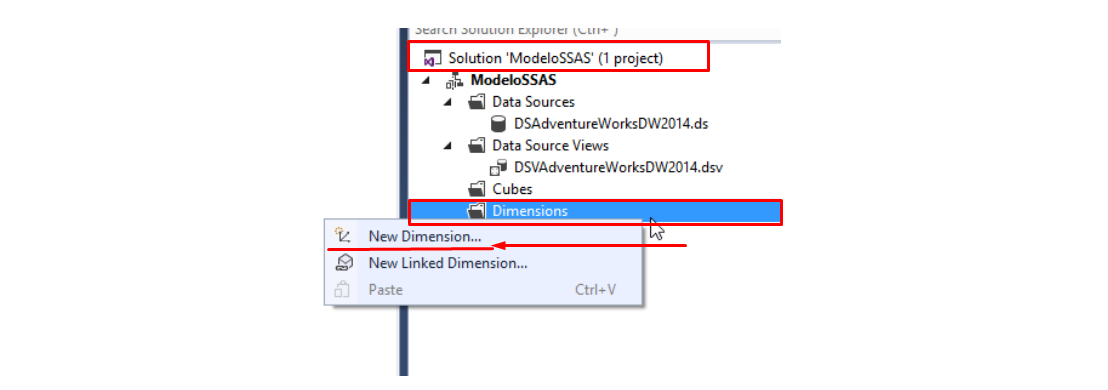
\includegraphics[width=\columnwidth]{./Imagenes/img2_3}
	\end{center}	


\item Eliminaremos el atributo EnglishProductName y renombraremos el atributo Product Key por Product, Procesamos la dimensión DimProduct.

\item Una vez procesada la dimensión nos volvemos a Reconcetar al mismo. Si ahora consultamos el atributo Product obtendremos lo siguiente:

	\begin{center}
	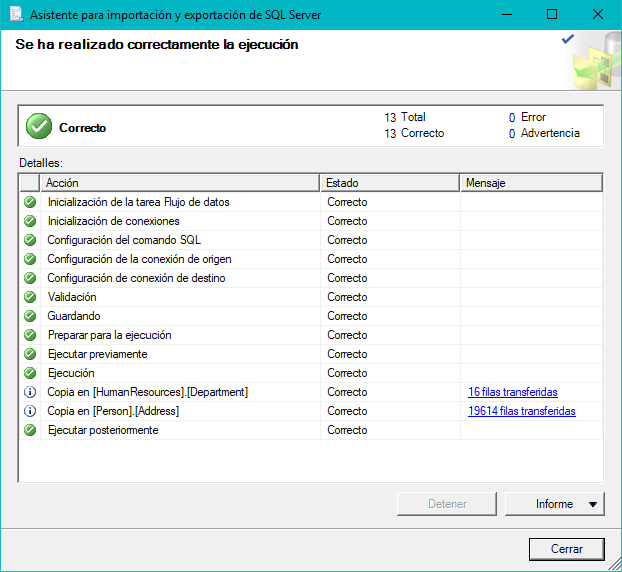
\includegraphics[width=\columnwidth]{./Imagenes/img3_3}
    \end{center}	



\end{itemize}
		
\include{Secciones/Actividad05}

\end{document}
